\section{State-of-the-Art}
	\tableofcontents[currentsection]
	
	\begin{comment}
	
	\begin{frame}{High-Performance FPGA-Based CNN Accelerator With Block-Floating-Point Arithmetic}
		\centering
		\begin{figure}
			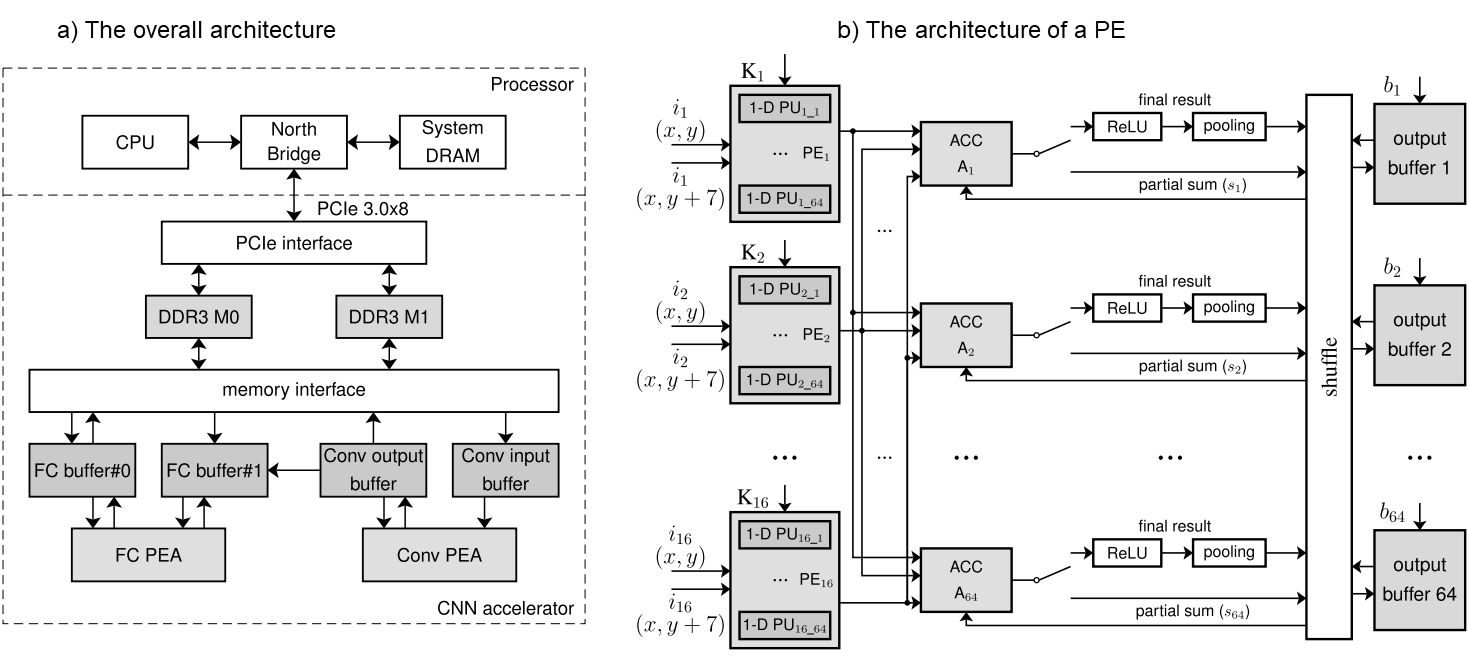
\includegraphics[width=\textwidth]{../figures/3_g.png}
			\caption{(a) System architecture. (b) Processing element array.}
		\end{figure}
	\end{frame}
	
	\begin{frame}{A 200MHZ 202.4GFLOPS@10.8W VGG16 Accelerator in Xilinx VX690T}
		\centering
		\begin{figure}
			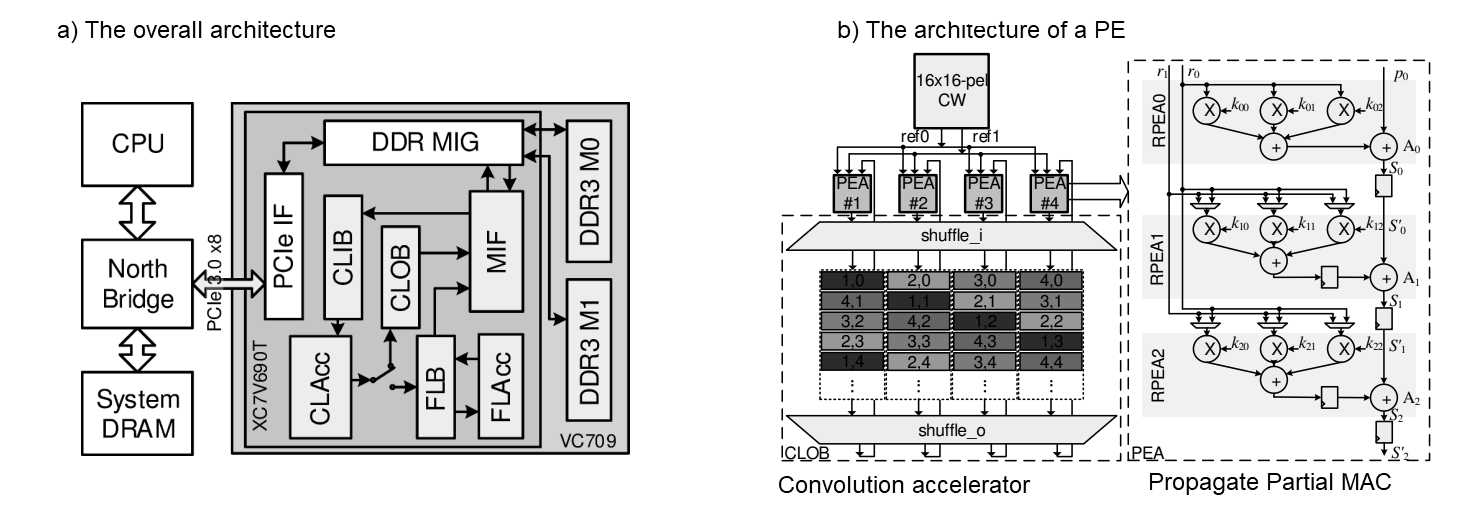
\includegraphics[width=\textwidth]{../figures/1_g.png}
			\caption{(a) System architecture. (b) Convolution accelerator.}
		\end{figure}
	\end{frame}
	
	\begin{frame}{Low-precision Floating-point Arithmetic for High-performance FPGA-based CNN Acceleration}
		\centering
		\begin{figure}
			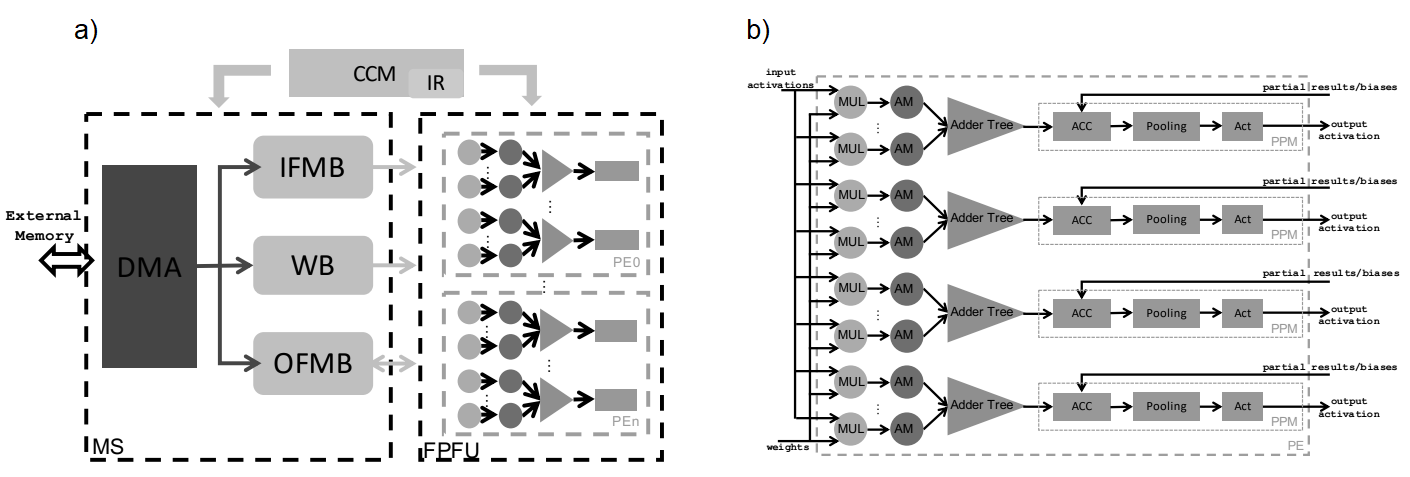
\includegraphics[width=\textwidth]{../figures/2_g.png}
			\caption{(a) System architecture. (b) Processing element.}
		\end{figure}
	\end{frame}

	\begin{frame}{CNN Hardware Acceleration on a Low-Power and Low-Cost APSoC}
	\centering
	\begin{figure}
		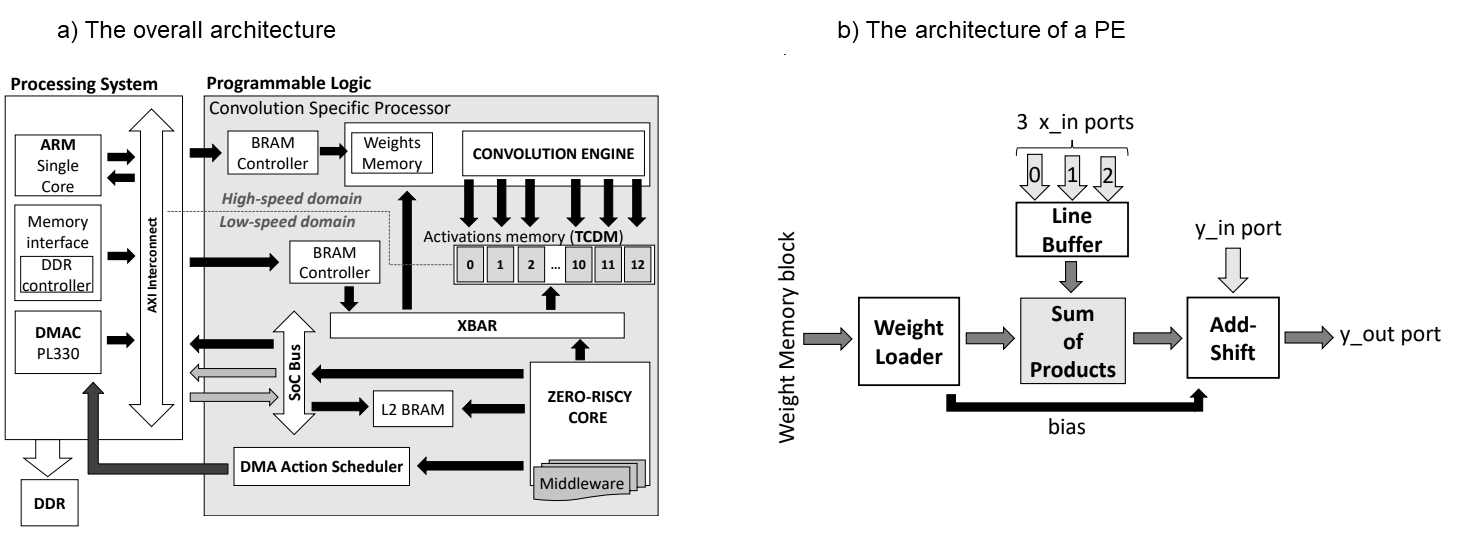
\includegraphics[width=\textwidth]{../figures/4_g.png}
		\caption{(a) System architecture. (b) Convolution engine.}
	\end{figure}
	\end{frame}
	
	\end{comment}
	
	
\begin{frame}{Limitations of State-of-the-Art in Low-Power Neural Network Accelerators}
	\begin{itemize}
		\item<1-> \textbf{Spike-by-Spike Neural Networks:}
		\begin{itemize}
			\item<2-> \alert{Quantization Challenges:} Struggles with reduced number representations (8-bit and 4-bit).
			\item<3-> \alert{Deployment Frameworks:} Lack of deployment strategies for IoT and TinyML applications.
			\item<4-> \alert{Design Methodologies:} Lack of effective low-power accelerator design methodologies to realize deployment.
		\end{itemize}
		\item<5-> \textbf{Convolutional Neural Networks:}
		\begin{itemize}
			\item<6-> \alert{Floating-Point Design:} Research gap in floating-point methodologies for resource-constrained IoT and TinyML applications.
			\item<7-> \alert{Reproducibility:} Deficiency in reproducible research, limiting validation and adoption.
		\end{itemize}
		\item<8-> \textbf{Aggressive Quantization:}
		\begin{itemize}
			\item<9-> \alert{Computational Efficiency vs. Accuracy:} Enhances efficiency but often at the expense of significant accuracy degradation.
			\item<10-> \alert{Mission-Critical Applications:} Often unsuitable for applications requiring high reliability, safety, and quality-of-result.
			\item<11-> \alert{Compatibility and Portability:} Faces challenges in compatibility and portability across different computing platforms and ML frameworks.
		\end{itemize}
	\end{itemize}
\end{frame}